\documentclass[utf8]{beamer}

\usepackage{xltxtra}
\usepackage[main=russian,english]{babel}

\usetheme{Antibes}
\usecolortheme{orchid}

\setmainfont{Arial}
\setromanfont{Times New Roman}
\setsansfont{Arial}
\setmonofont{Courier New}
% далее идёт преамбула
\title{Вопросы подготовки и оформления РПП АО ЮТэйр}
\author{Белоконь Д.}

\begin{document}% начало презентации

\begin{frame}% первый слайд
\titlepage
\end{frame}

\begin{frame}{Нумерация пунктов}    
            \begin{itemize}
                    \item<1-> Нумерация абсолютно каждого пункта...
                    \item<1-> 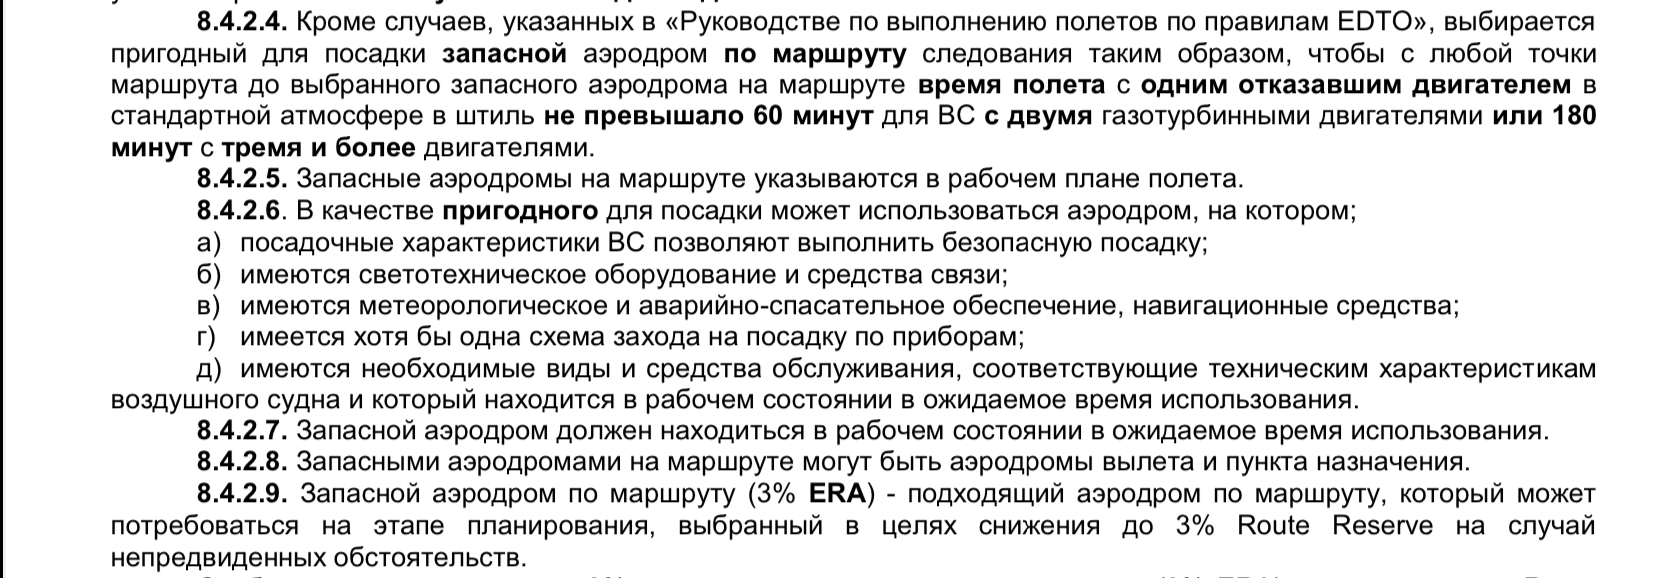
\includegraphics[width=0.8\textwidth]{Numeric1.png}
                    \item<2-> ...или отсутствие номеров
                    \item<2-> 
\includegraphics[width=0.8\textwidth]{Numeric3.png}
            \end{itemize}              
\end{frame}

\begin{frame}{Нумерация пунктов}    
        потеряна логика нумерации...
        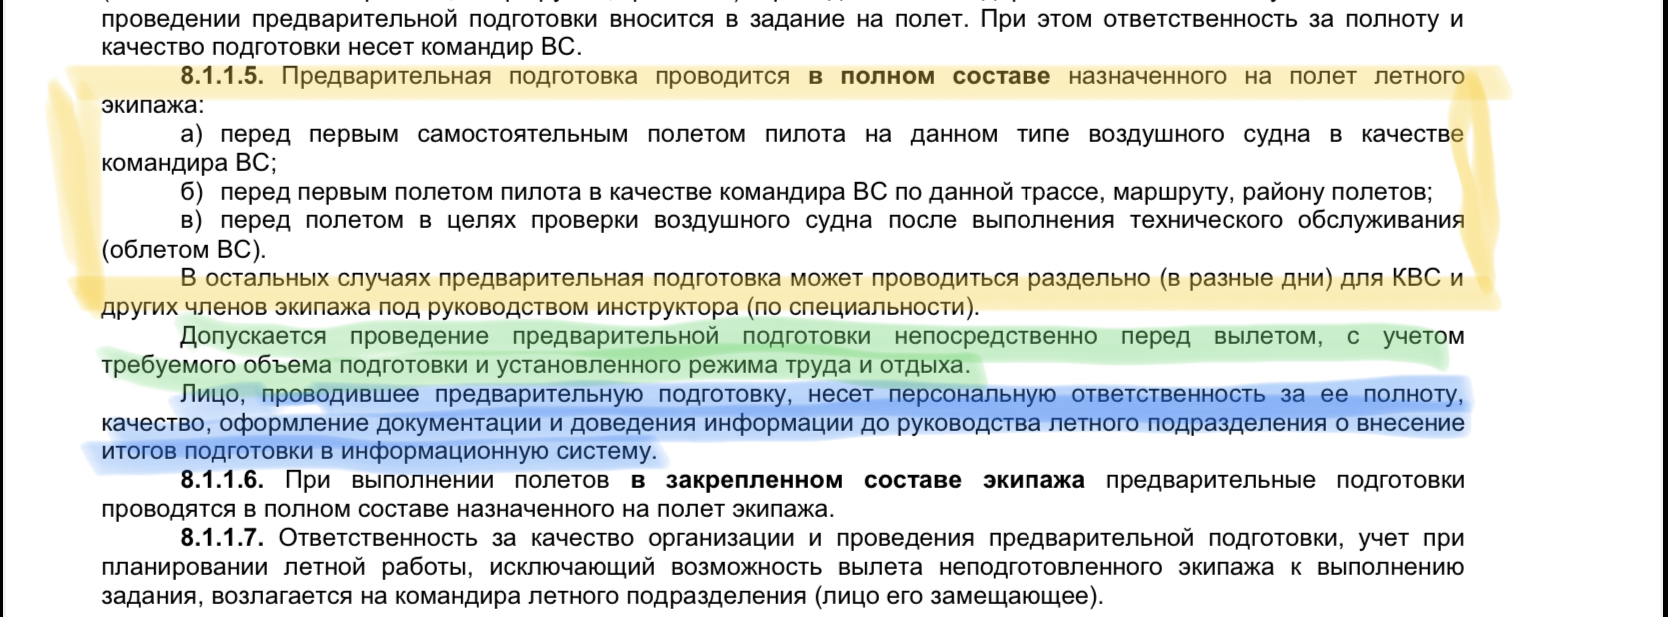
\includegraphics[width=0.8\textwidth]{Numeric4.png}            
\end{frame}

\begin{frame}{Нумерация пунктов}    
    повторение номеров...
    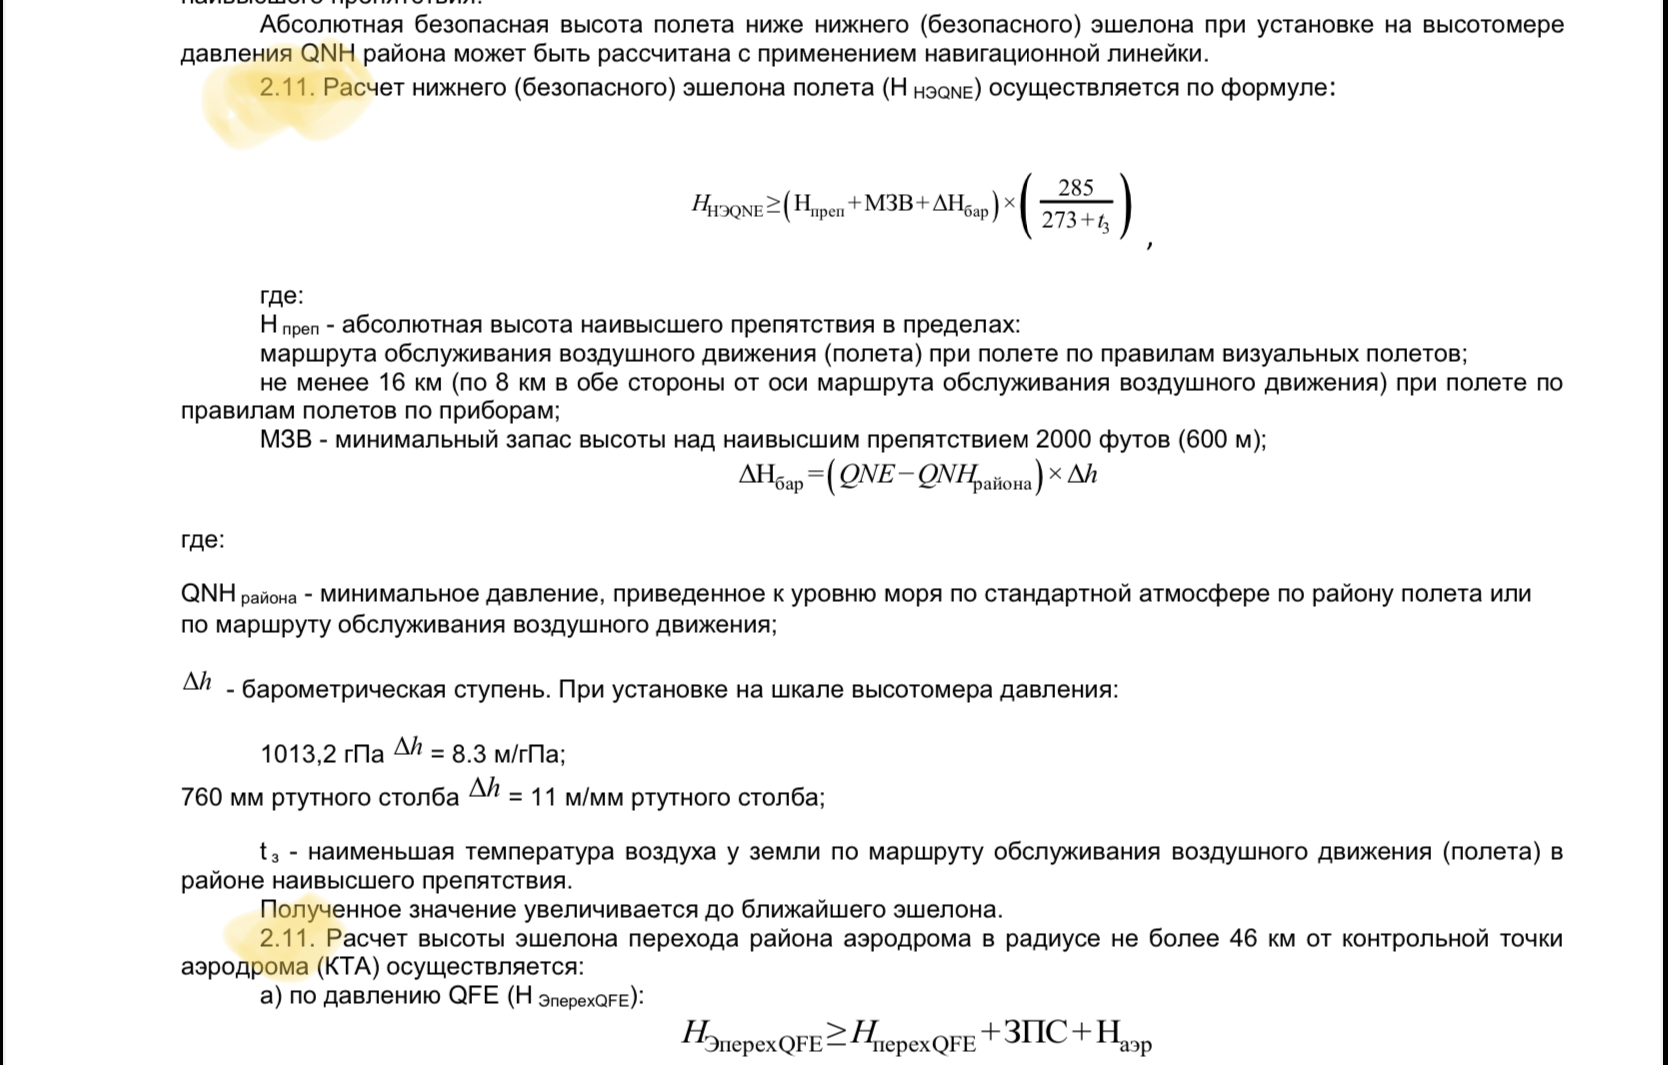
\includegraphics[width=0.8\textwidth]{Numeric2.png}            
\end{frame}


\begin{frame}{Нумерация таблиц}
    \begin{columns}[T,onlytextwidth]
            \begin{column}{0.48\textwidth}
                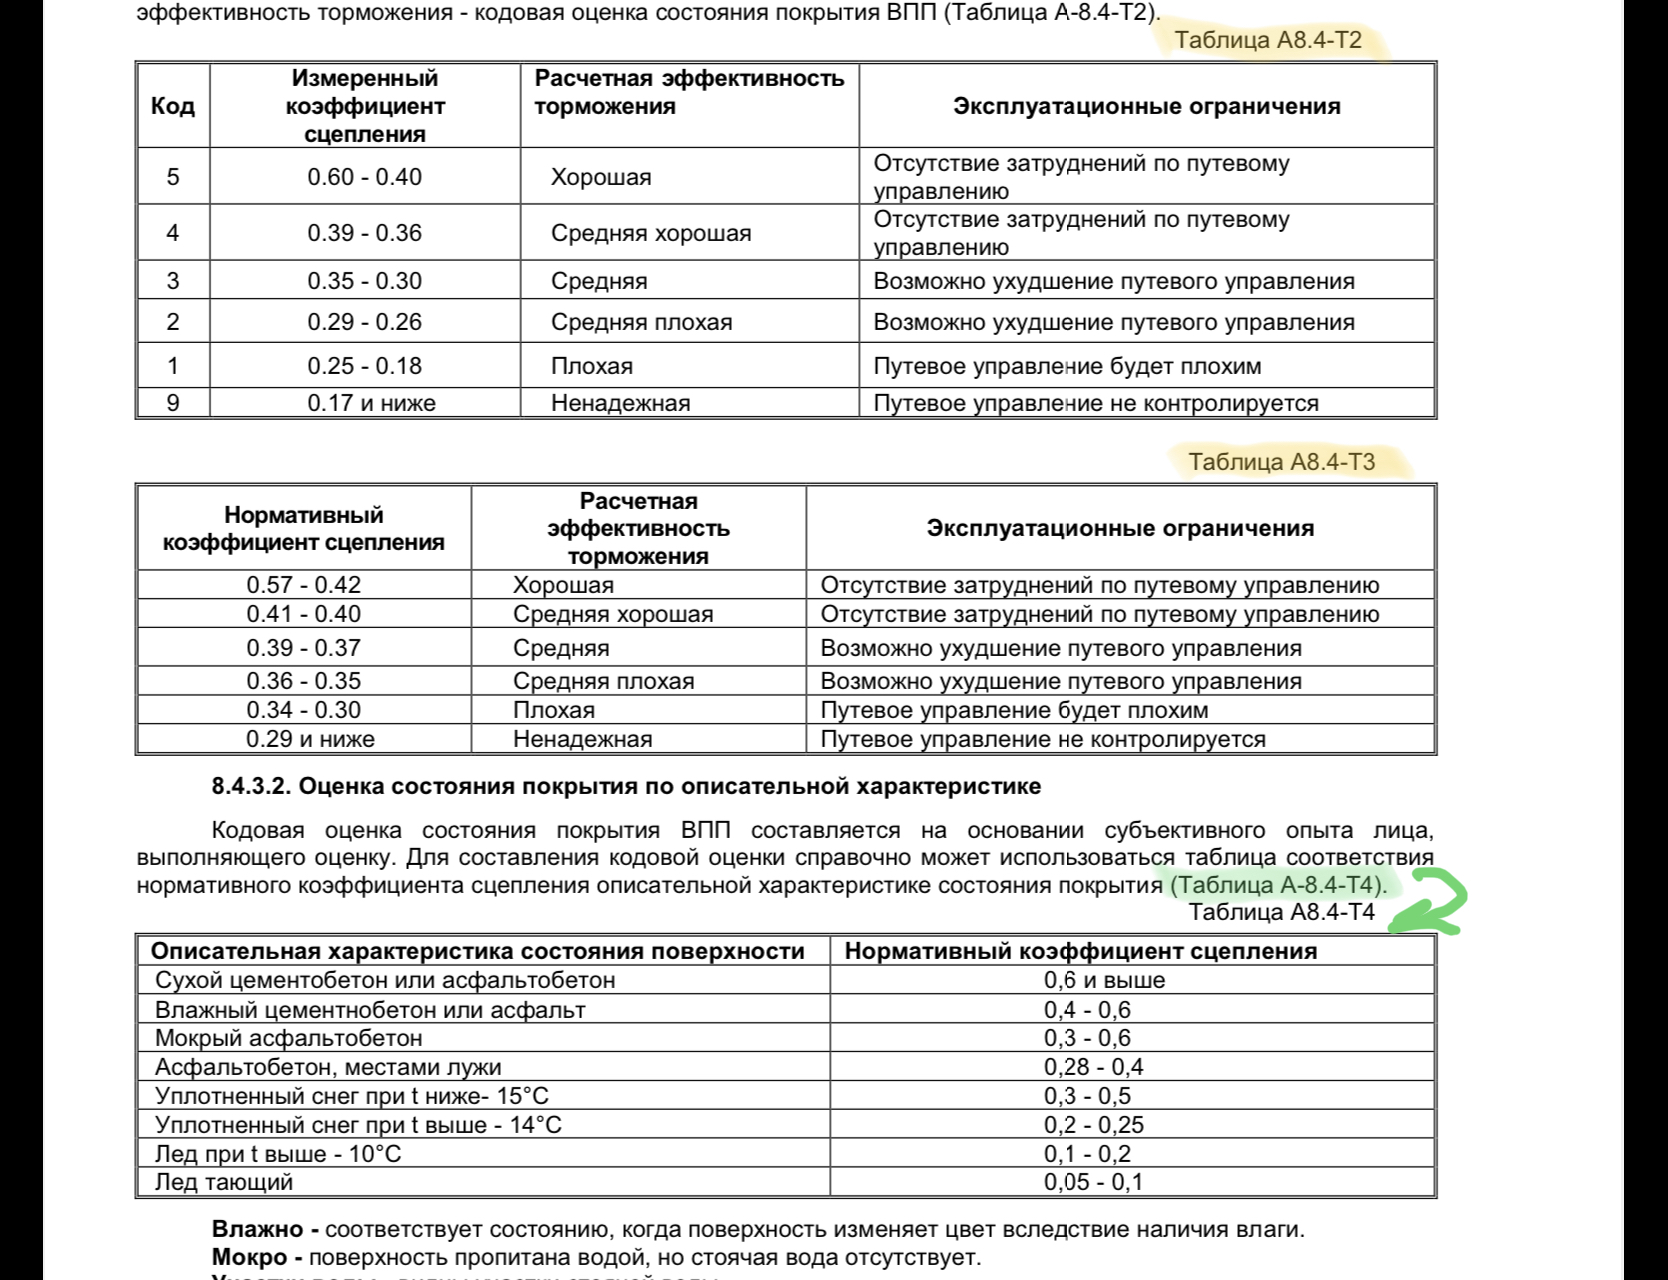
\includegraphics[width=0.8\textwidth]{Complex1.png}                                     
            \end{column}
            \begin{column}{0.48\textwidth}
                \begin{itemize}
                    \item<1-> Сложная в конструкции и запоминании
                    \item<2-> Излишние ссылки
                    \item<3-> В др.а/к:
                    \item<3-> 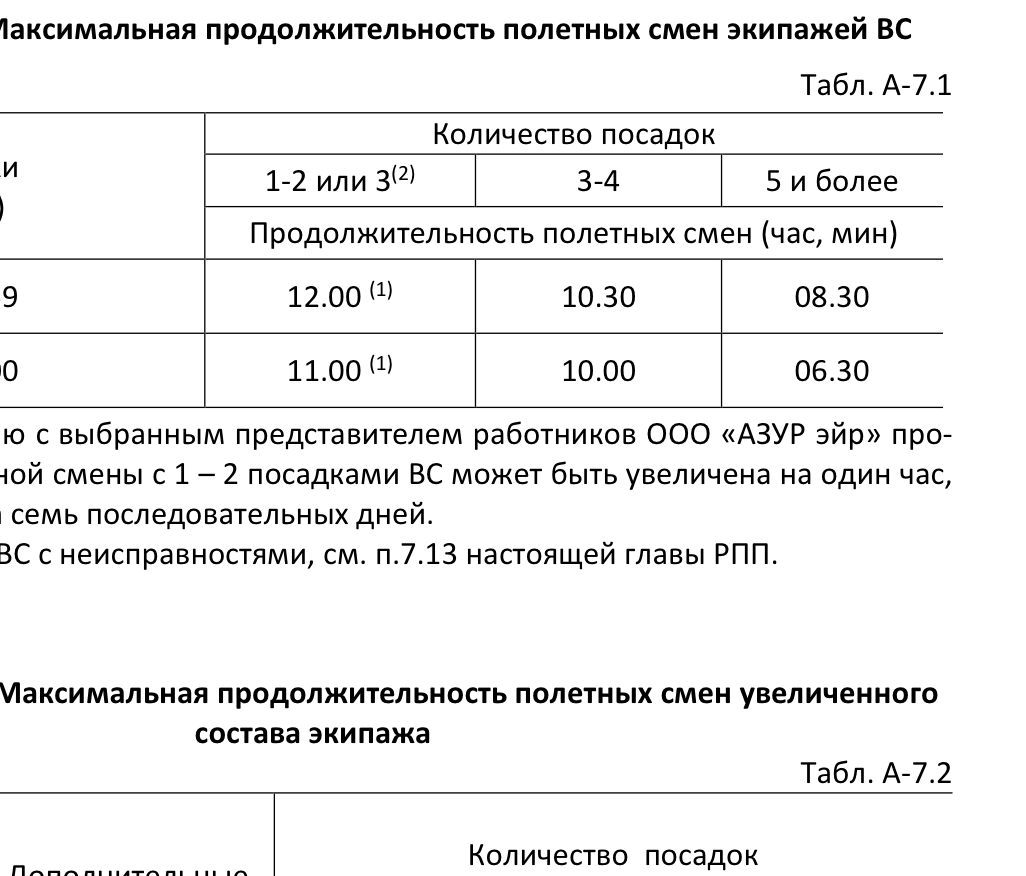
\includegraphics[width=0.8\textwidth]{AzurTables.png}
            \end{itemize}    
            \end{column}
    \end{columns}    
\end{frame}

\begin{frame}{Логика}  
    \begin{itemize}
        \item <1-> Ссылки на рядом находящиеся пункты:
        \item <1-> 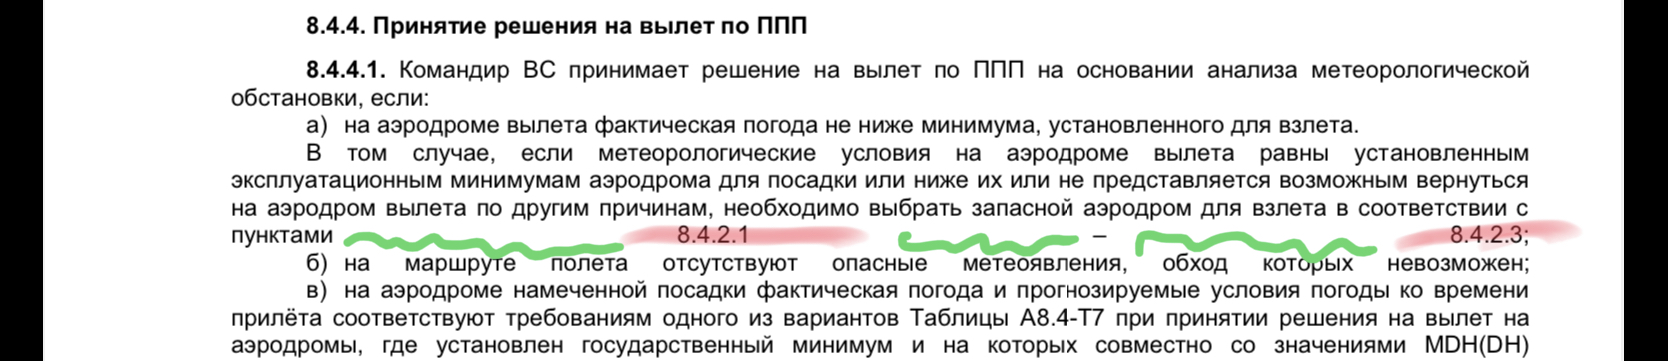
\includegraphics[width=0.8\textwidth]{Logic1.png} 
        \item <2-> Количество ссылок и ссылки на пункты в разных частях документа:
        \item <2-> 
\includegraphics[width=0.8\textwidth]{Logic2.png}
    \end{itemize}              
\end{frame}

\begin{frame}{Логика}  
    \begin{itemize}
        \item <1-> повтор формулировок по значениям:
        \item <1-> 
\includegraphics[width=0.8\textwidth]{Logic3.png} 
        \item <2-> копирование информации из Приложения 1 к этой же главе:
        \item <2-> 
\includegraphics[width=0.8\textwidth]{Logic5.png}
    \end{itemize}              
\end{frame}

\begin{frame}{Оформление}  
    \begin{itemize}
        \item <1-> Разделы и подразделы неотличимы:
        \item <1-> 
\includegraphics[width=0.8\textwidth]{Visual1.png} 
        \item <2-> висящие абзацы:
        \item <2-> 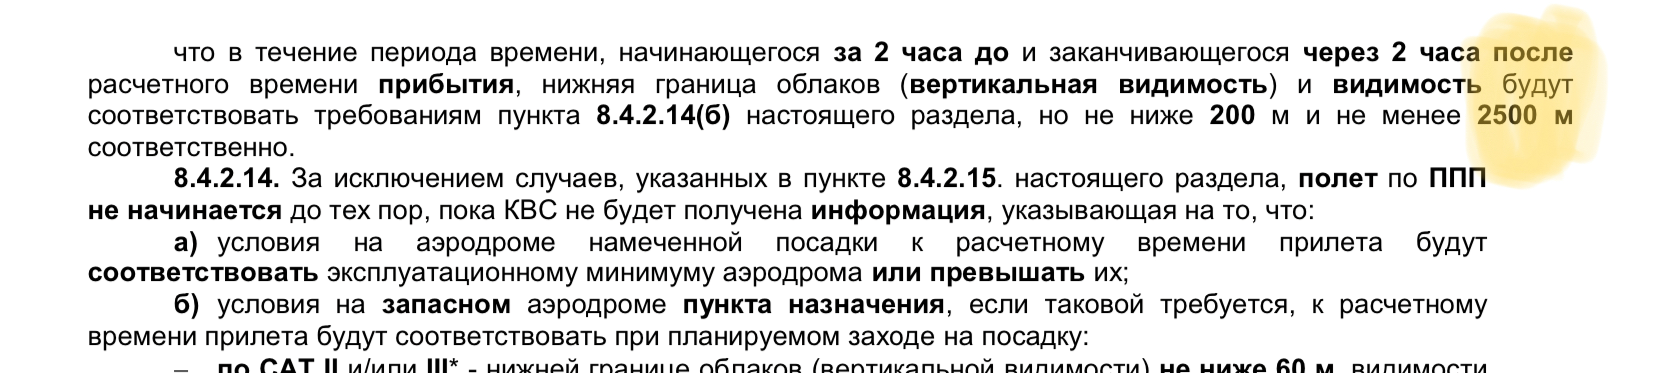
\includegraphics[width=0.8\textwidth]{Visual2.png}
    \end{itemize}              
\end{frame}

\begin{frame}{Оформление}  
    \begin{itemize}
        \item <1-> визуальная перегрузка списка:
        \item <1-> 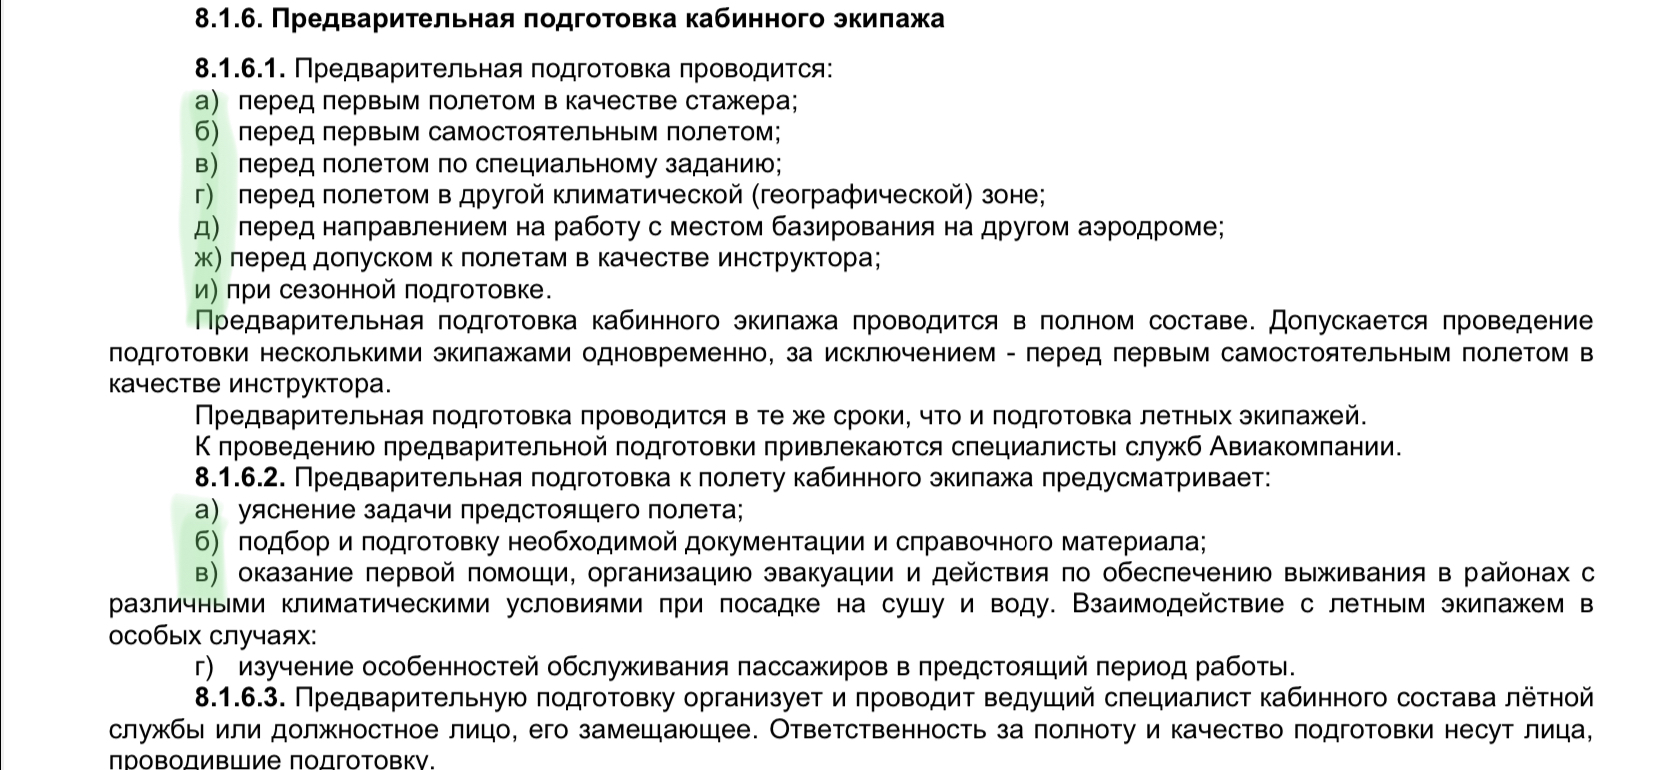
\includegraphics[width=0.8\textwidth]{Visual4.png} 
        \item <2-> неотличимые списки, все на одном уровне:
        \item <2-> 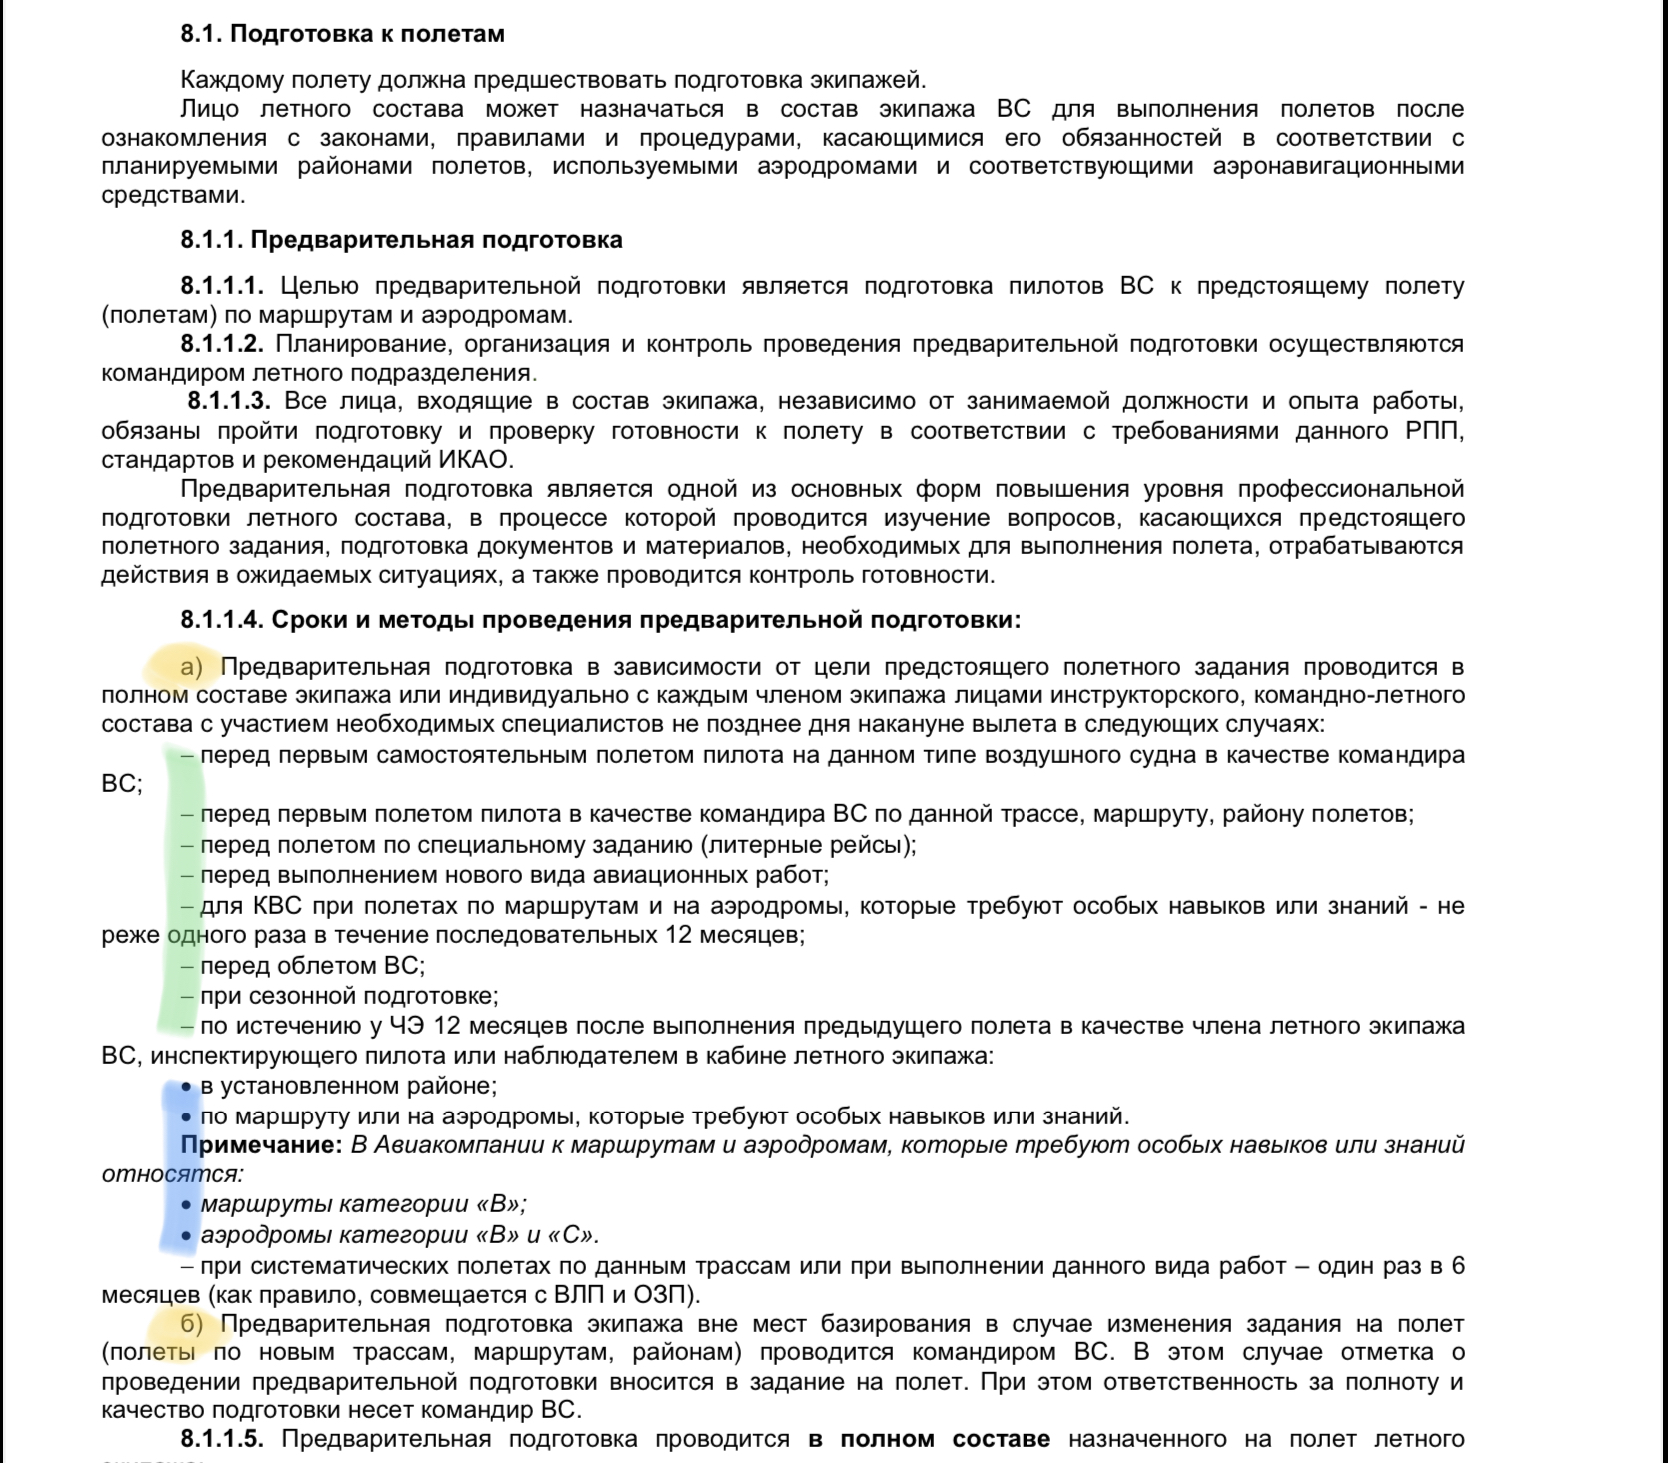
\includegraphics[width=0.8\textwidth]{Visual5.png}
    \end{itemize}              
\end{frame}

\begin{frame}{...}  
    \begin{itemize}
        \item <1-> большинство замечаний поможет устранить...
        \item <2-> \huge \LaTeX
    \end{itemize}              
\end{frame}

\begin{frame}{LaTeX}  
    \begin{itemize}
        \item <1-> Полностью АВТОМАТИЧЕСКОЕ и интерактивное оглавление:
        \item <1-> 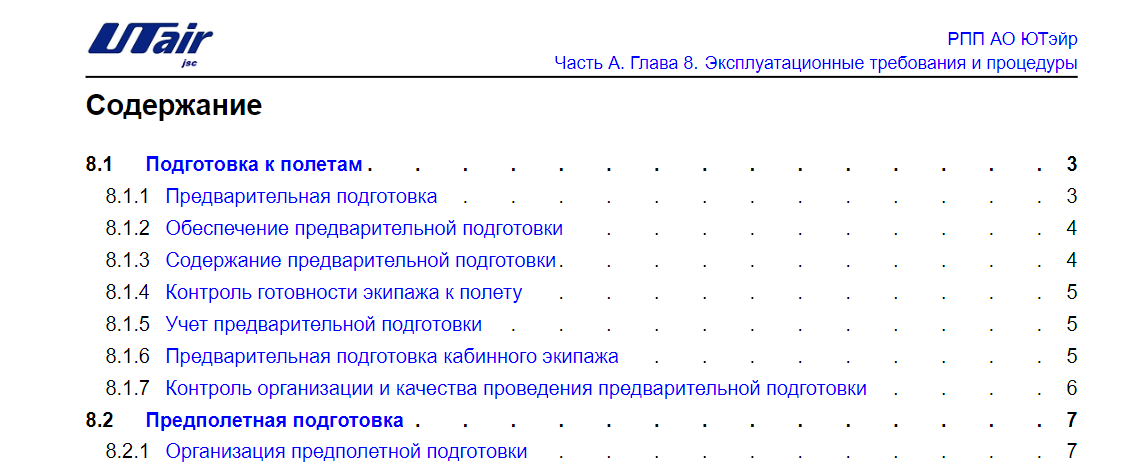
\includegraphics[width=0.8\textwidth]{lt01-contents.png} 
        \item <2-> автоматическое выравнивание:
        \item <2-> 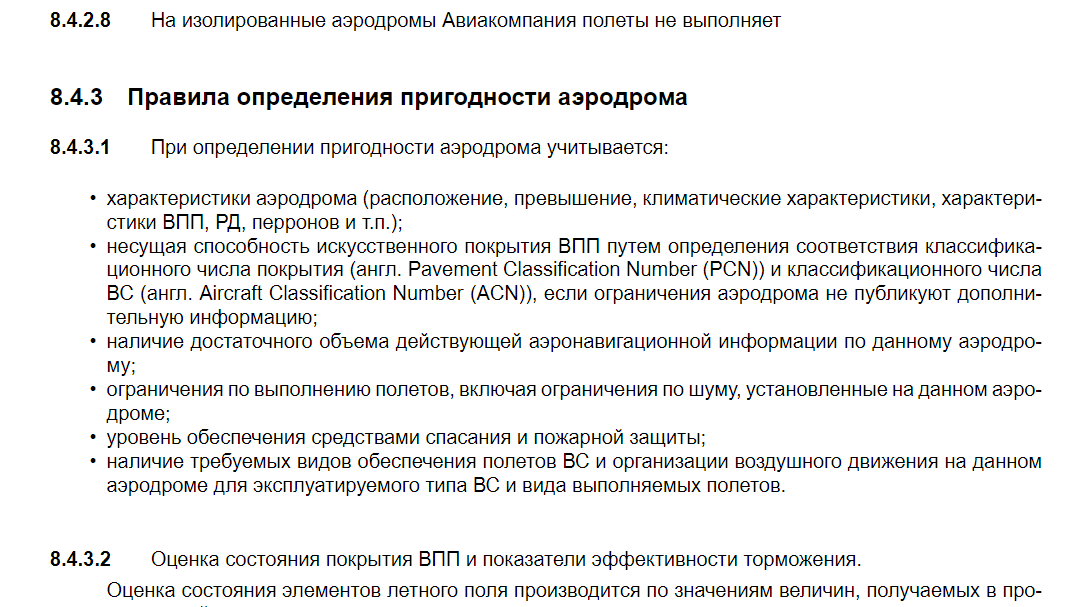
\includegraphics[width=0.8\textwidth]{lt05-alignes.png}
    \end{itemize}              
\end{frame}

\begin{frame}{LaTeX}  
    \begin{itemize}
        \item <1-> АВТОМАТИЧЕСКОЕ выравнивание и нумерация списков:
        \item <2-> 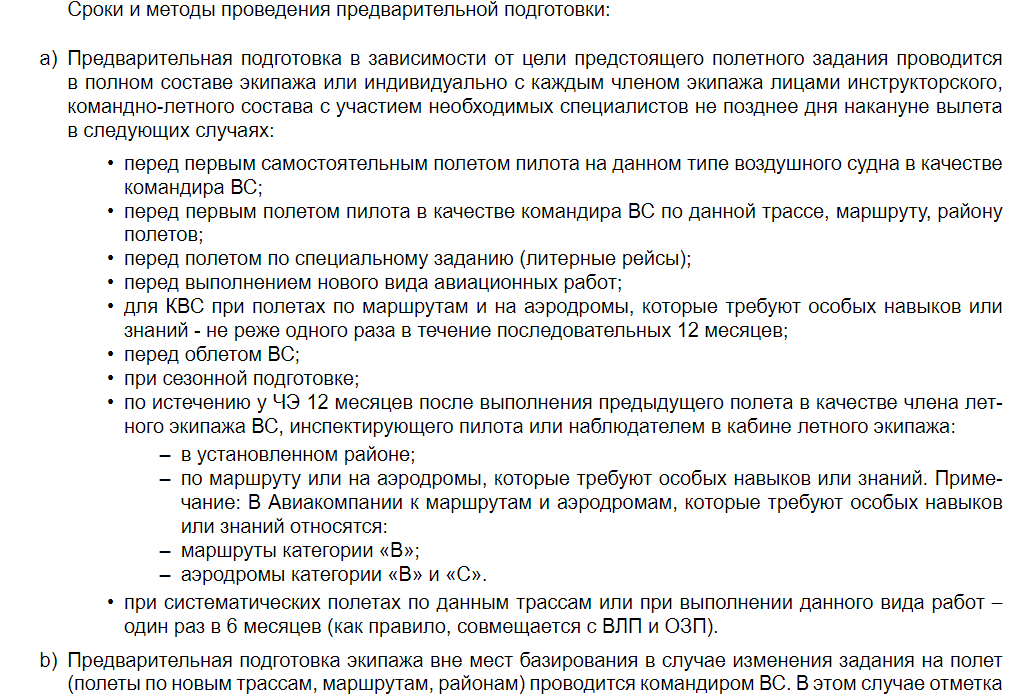
\includegraphics[width=0.8\textwidth]{lt02 - lists.png} 
    \end{itemize}              
\end{frame}

\begin{frame}{LaTeX}  
    \begin{itemize}
        \item <1-> возможность автоматического расположения и маркирования изменений:
        \item <2-> 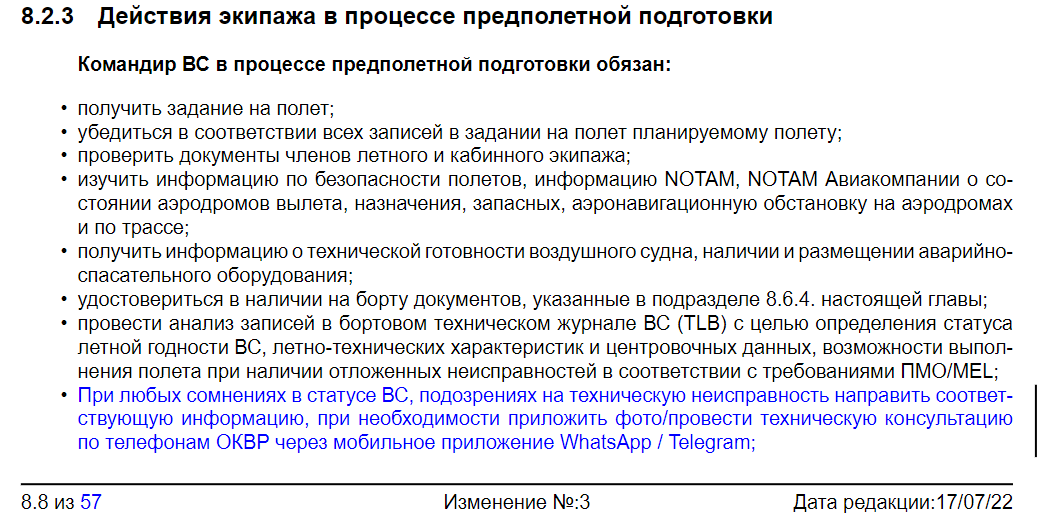
\includegraphics[width=0.8\textwidth]{lt03-changes.png}
    \end{itemize}              
\end{frame}

\begin{frame}{LaTeX}  
    \begin{itemize}
        \item <1-> возможность автоматического отслеживания и изменения ссылок:
        \item <2-> 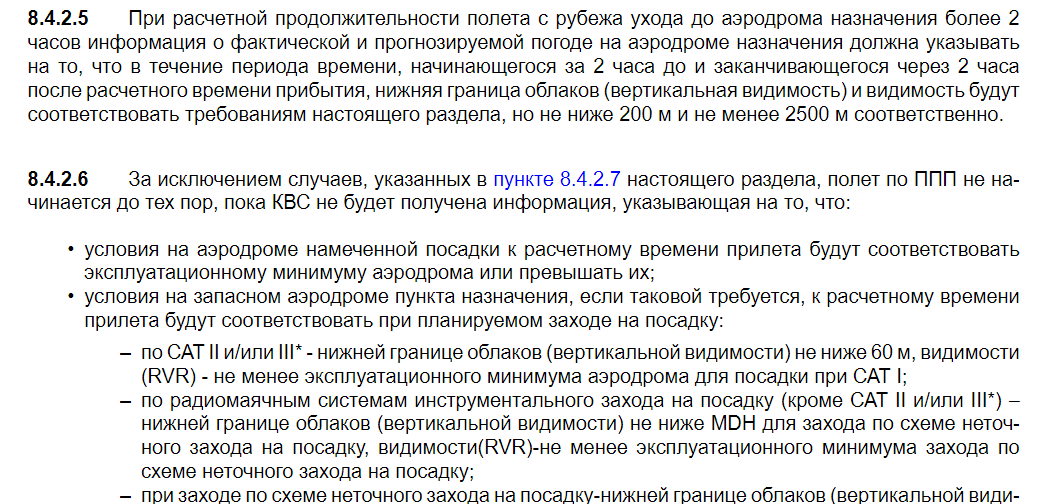
\includegraphics[width=0.8\textwidth]{lt04-links.png}
    \end{itemize}              
\end{frame}

\begin{frame}{LaTeX}  
    \begin{itemize}
        \item <1-> возможность изменения формата документа в течении минут:
        \item <2-> А4: 
\includegraphics[width=0.8\textwidth]{lt06-a4.png}
        \item <3-> А5: 
\includegraphics[width=0.8\textwidth]{lt07-a5.png}
    \end{itemize}              
\end{frame}

\begin{frame}{LaTeX}  
    Главный документ, структура:

    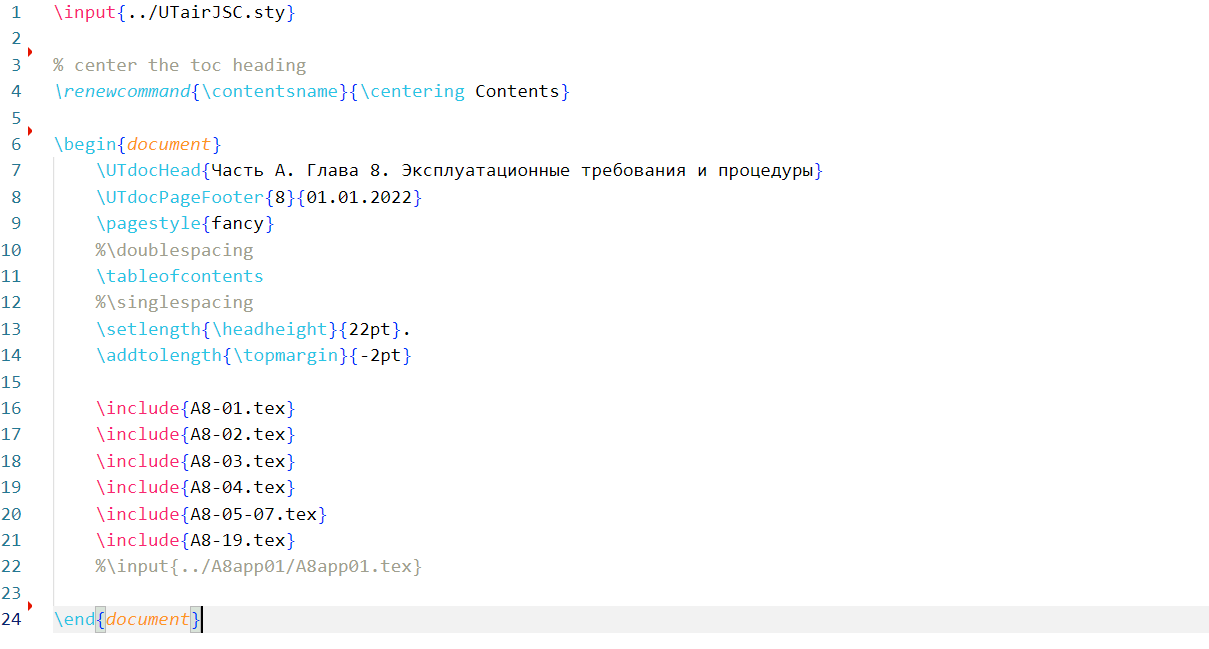
\includegraphics[width=\textwidth]{lt08-a8-1.png}           
\end{frame}
\begin{frame}{LaTeX}  
    Часть документа, заголовки и параграфы:

    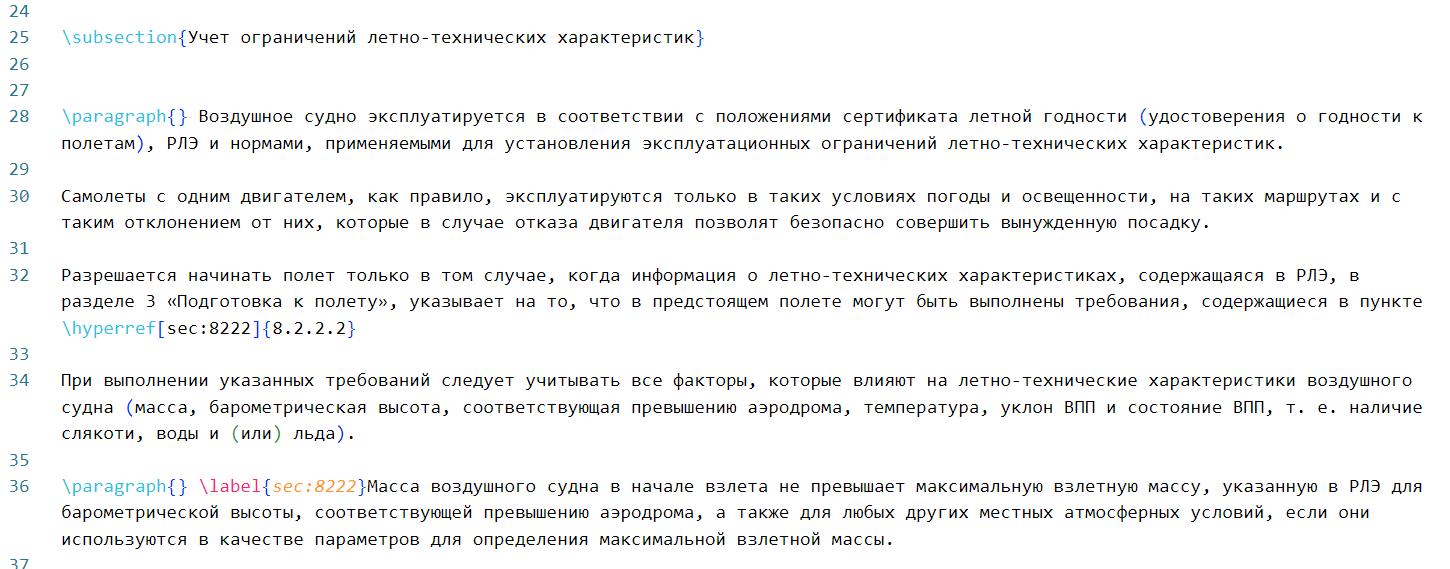
\includegraphics[width=\textwidth]{lt09-a8-2.png}           
\end{frame}
\begin{frame}{LaTeX}  
    Списки:
 
    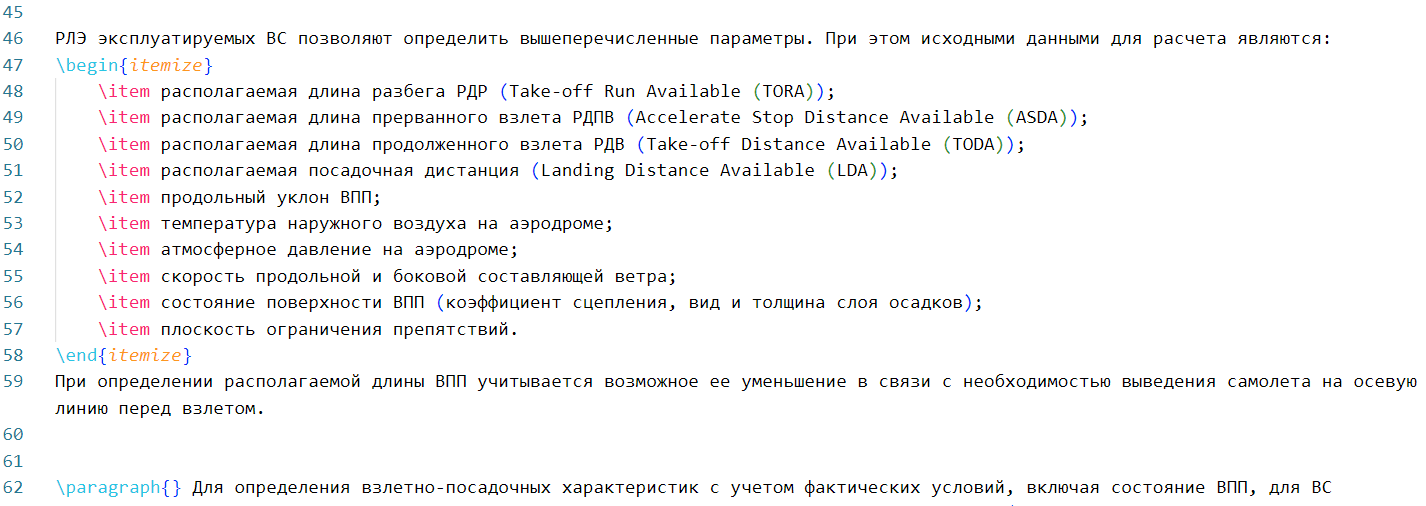
\includegraphics[width=\textwidth]{lt10-a8-3.png}           
\end{frame}
\begin{frame}{LaTeX}  
    Таблицы:

    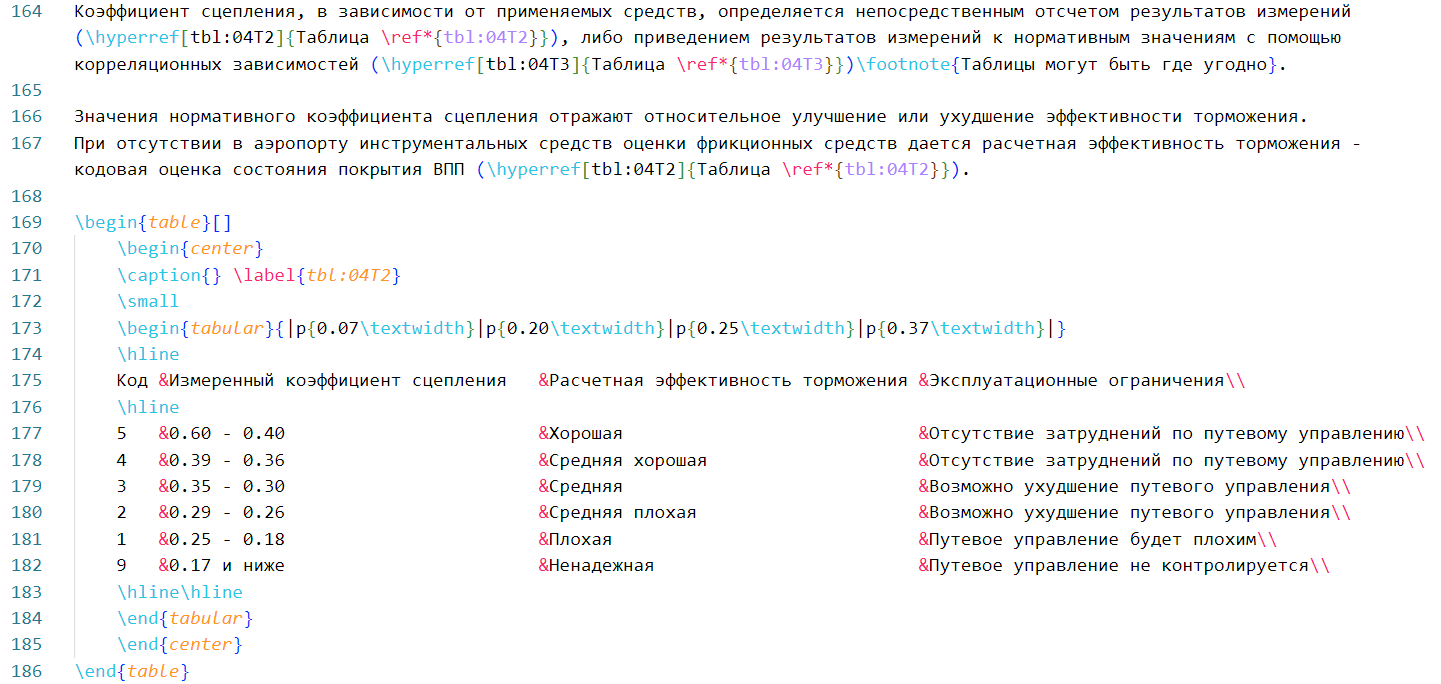
\includegraphics[width=\textwidth]{lt11-a8-4.png}           
\end{frame}
\begin{frame}{LaTeX}  
    Таблицы:

    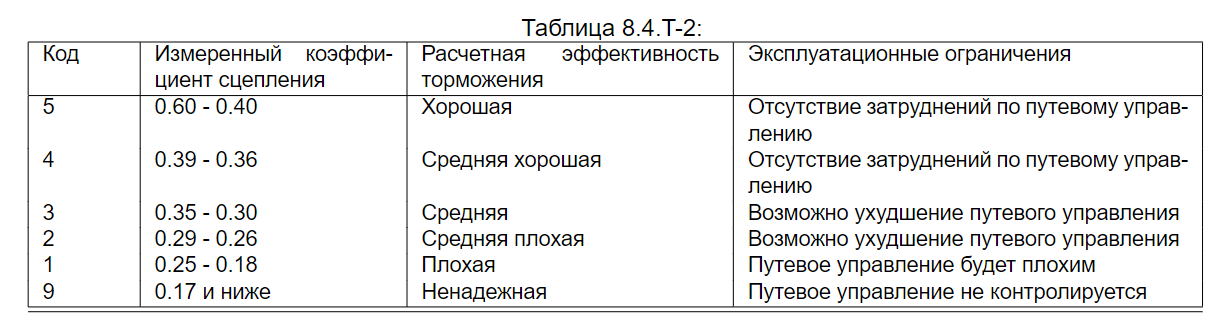
\includegraphics[width=\textwidth]{lt12-a8-table.png}           
\end{frame}

\end{document}